\interlude[1]{Hybridization}

\begin{frame}{In the following slides, you will learn…}
\hypertarget{you-will-learn-hybrid}{}
  …that hybrid, practical, post-quantum cryptography is built by combining pre-quantum and post-quantum primitives.

  \vspace{2em}
  …that key encapsulation methods can be combined, rendering a protocol like Rosenpass useful in pre-quantum as well
  as post-quantum settings.

  \vspace{2em}
  …why combining protocols like WireGuard and Rosenpass directly is still useful to enable code-reuse and to avoid
  loosing trust in established systems like WireGuard.
\end{frame}

\begin{frame}{Combining two KEMs with the GHP-Combiner}
  \hypertarget{ghp-combiner}{}
  \centering
  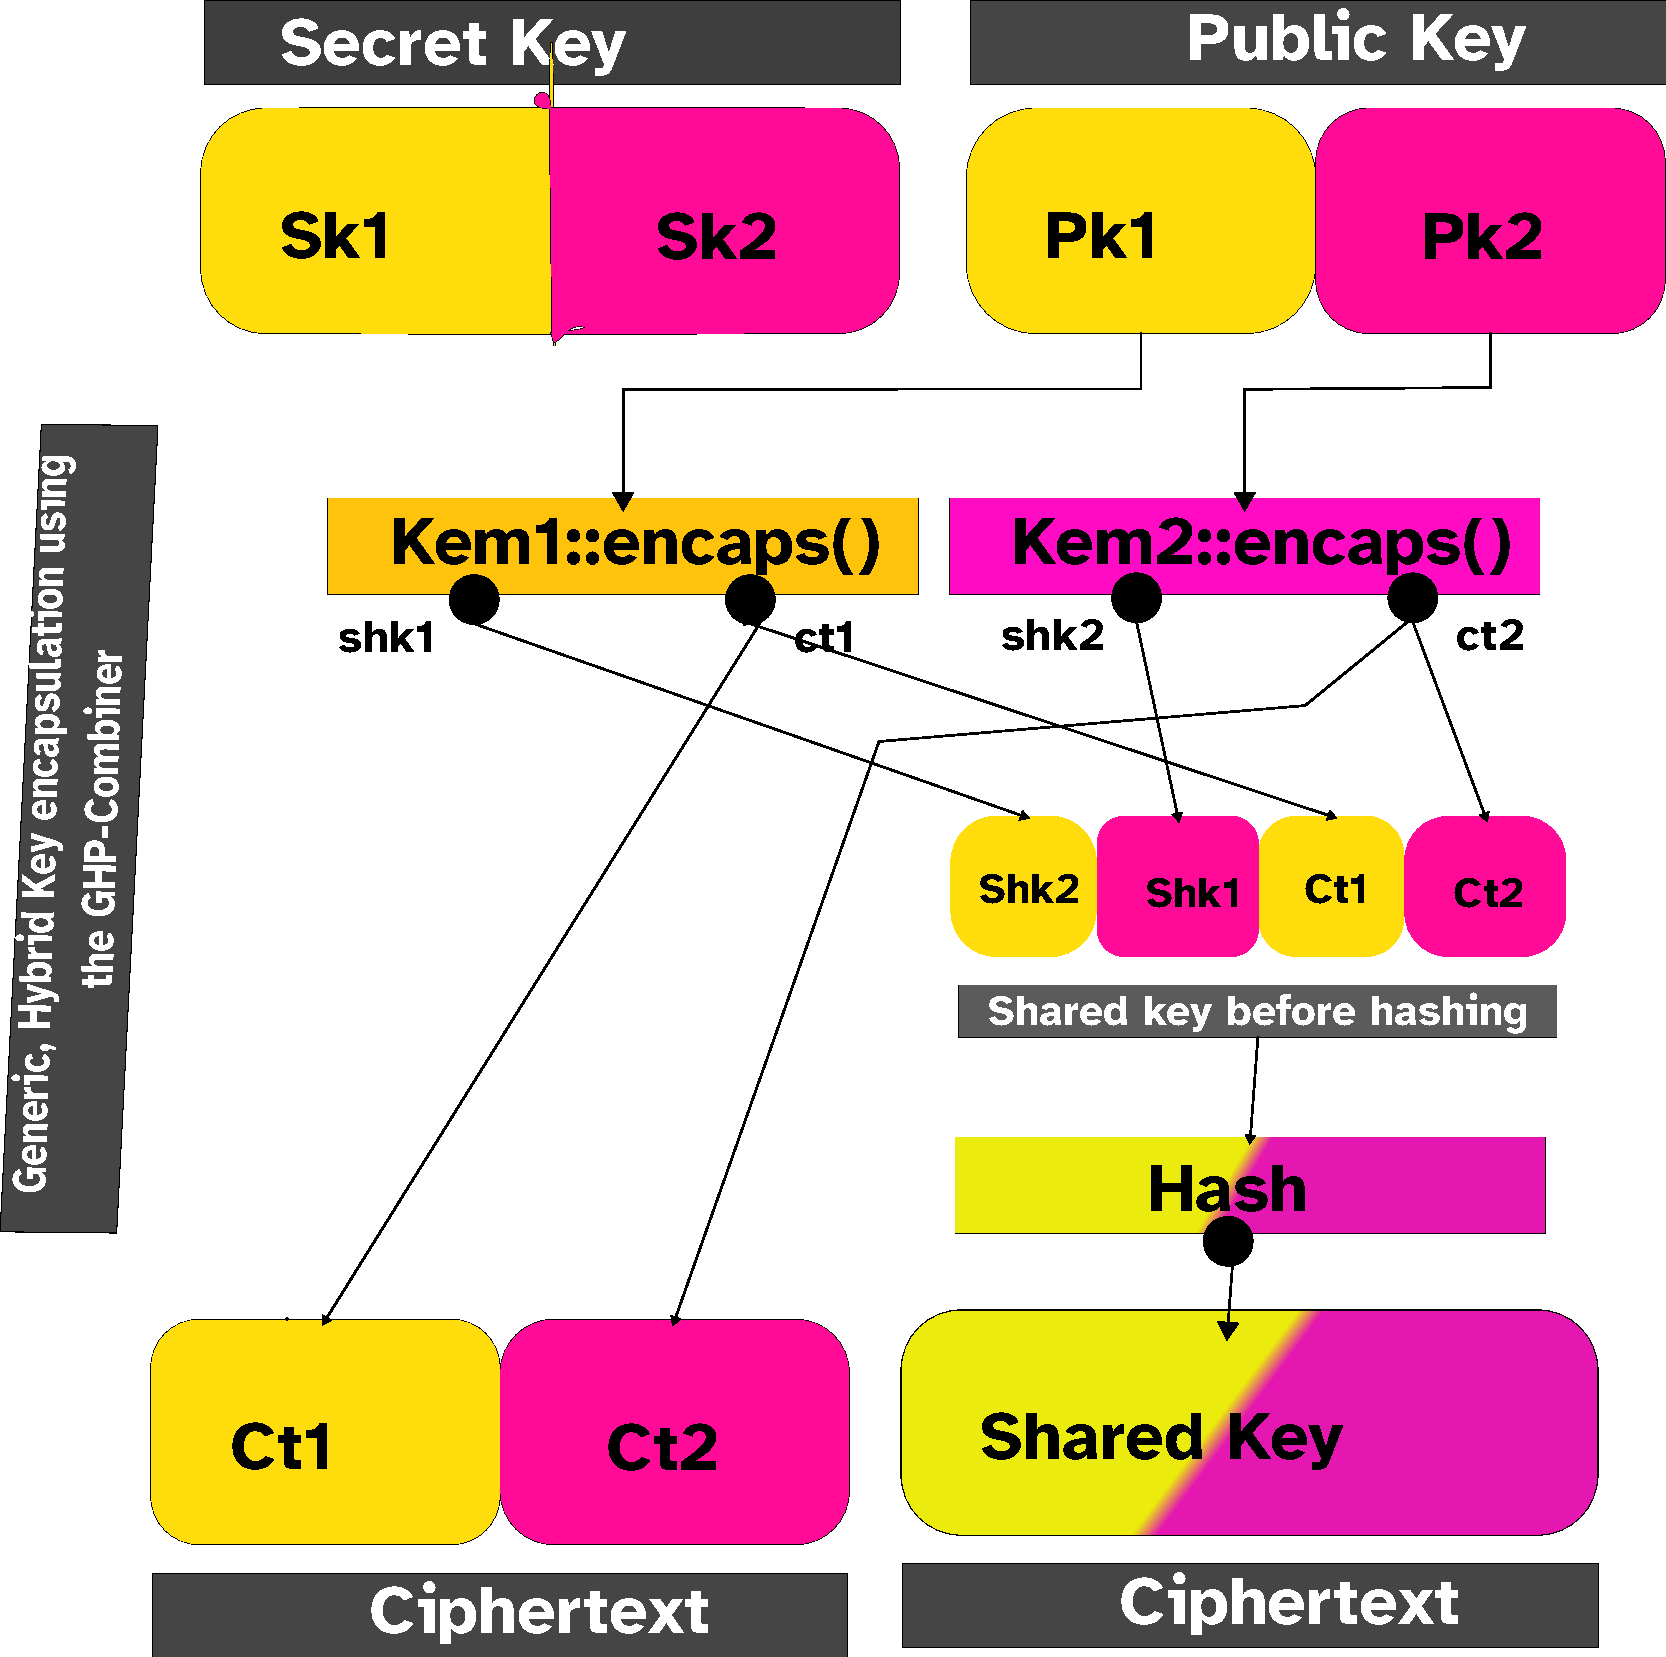
\includegraphics[height=.85\textheight]{graphics/ghp-combiner.pdf}
\end{frame}

\begin{frame}{Turning a NIKE into a KEM}
  \hypertarget{dhkem}{}
  \centering
    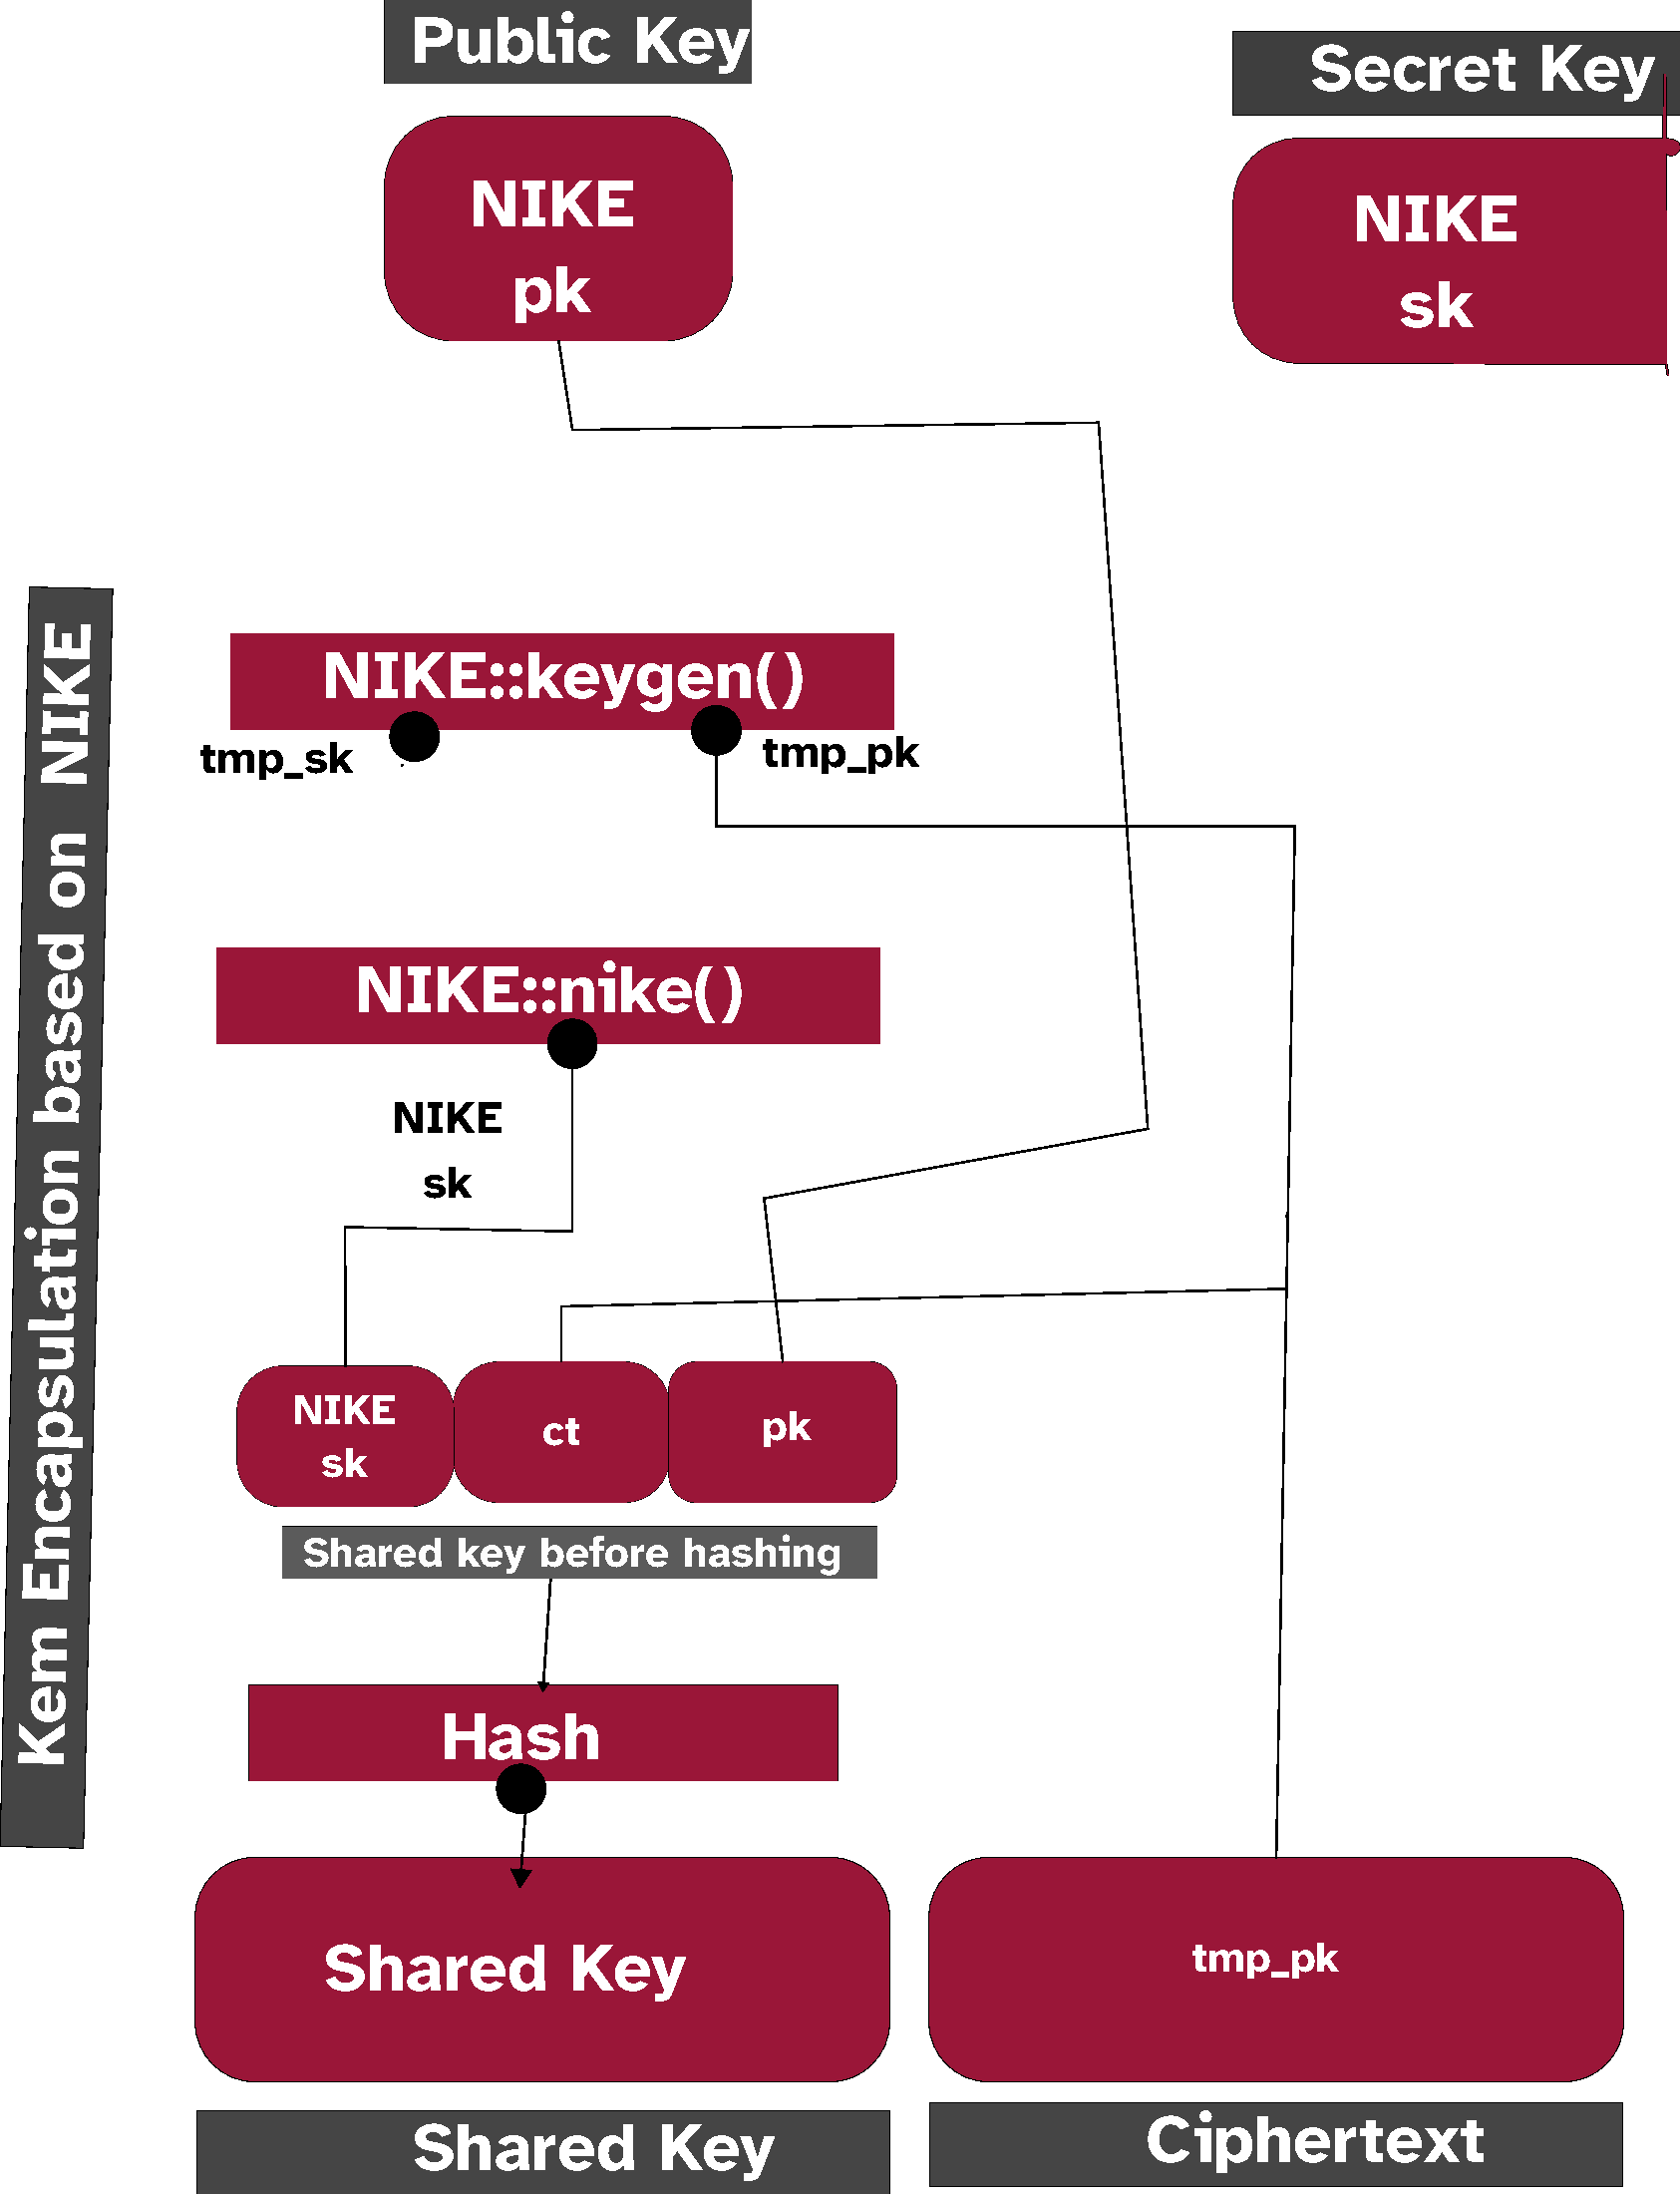
\includegraphics[height=.85\textheight]{graphics/dhkem.pdf}
\end{frame}

\begin{frame}{X-Wing}
  \hypertarget{x-wing}{}
  \centering
  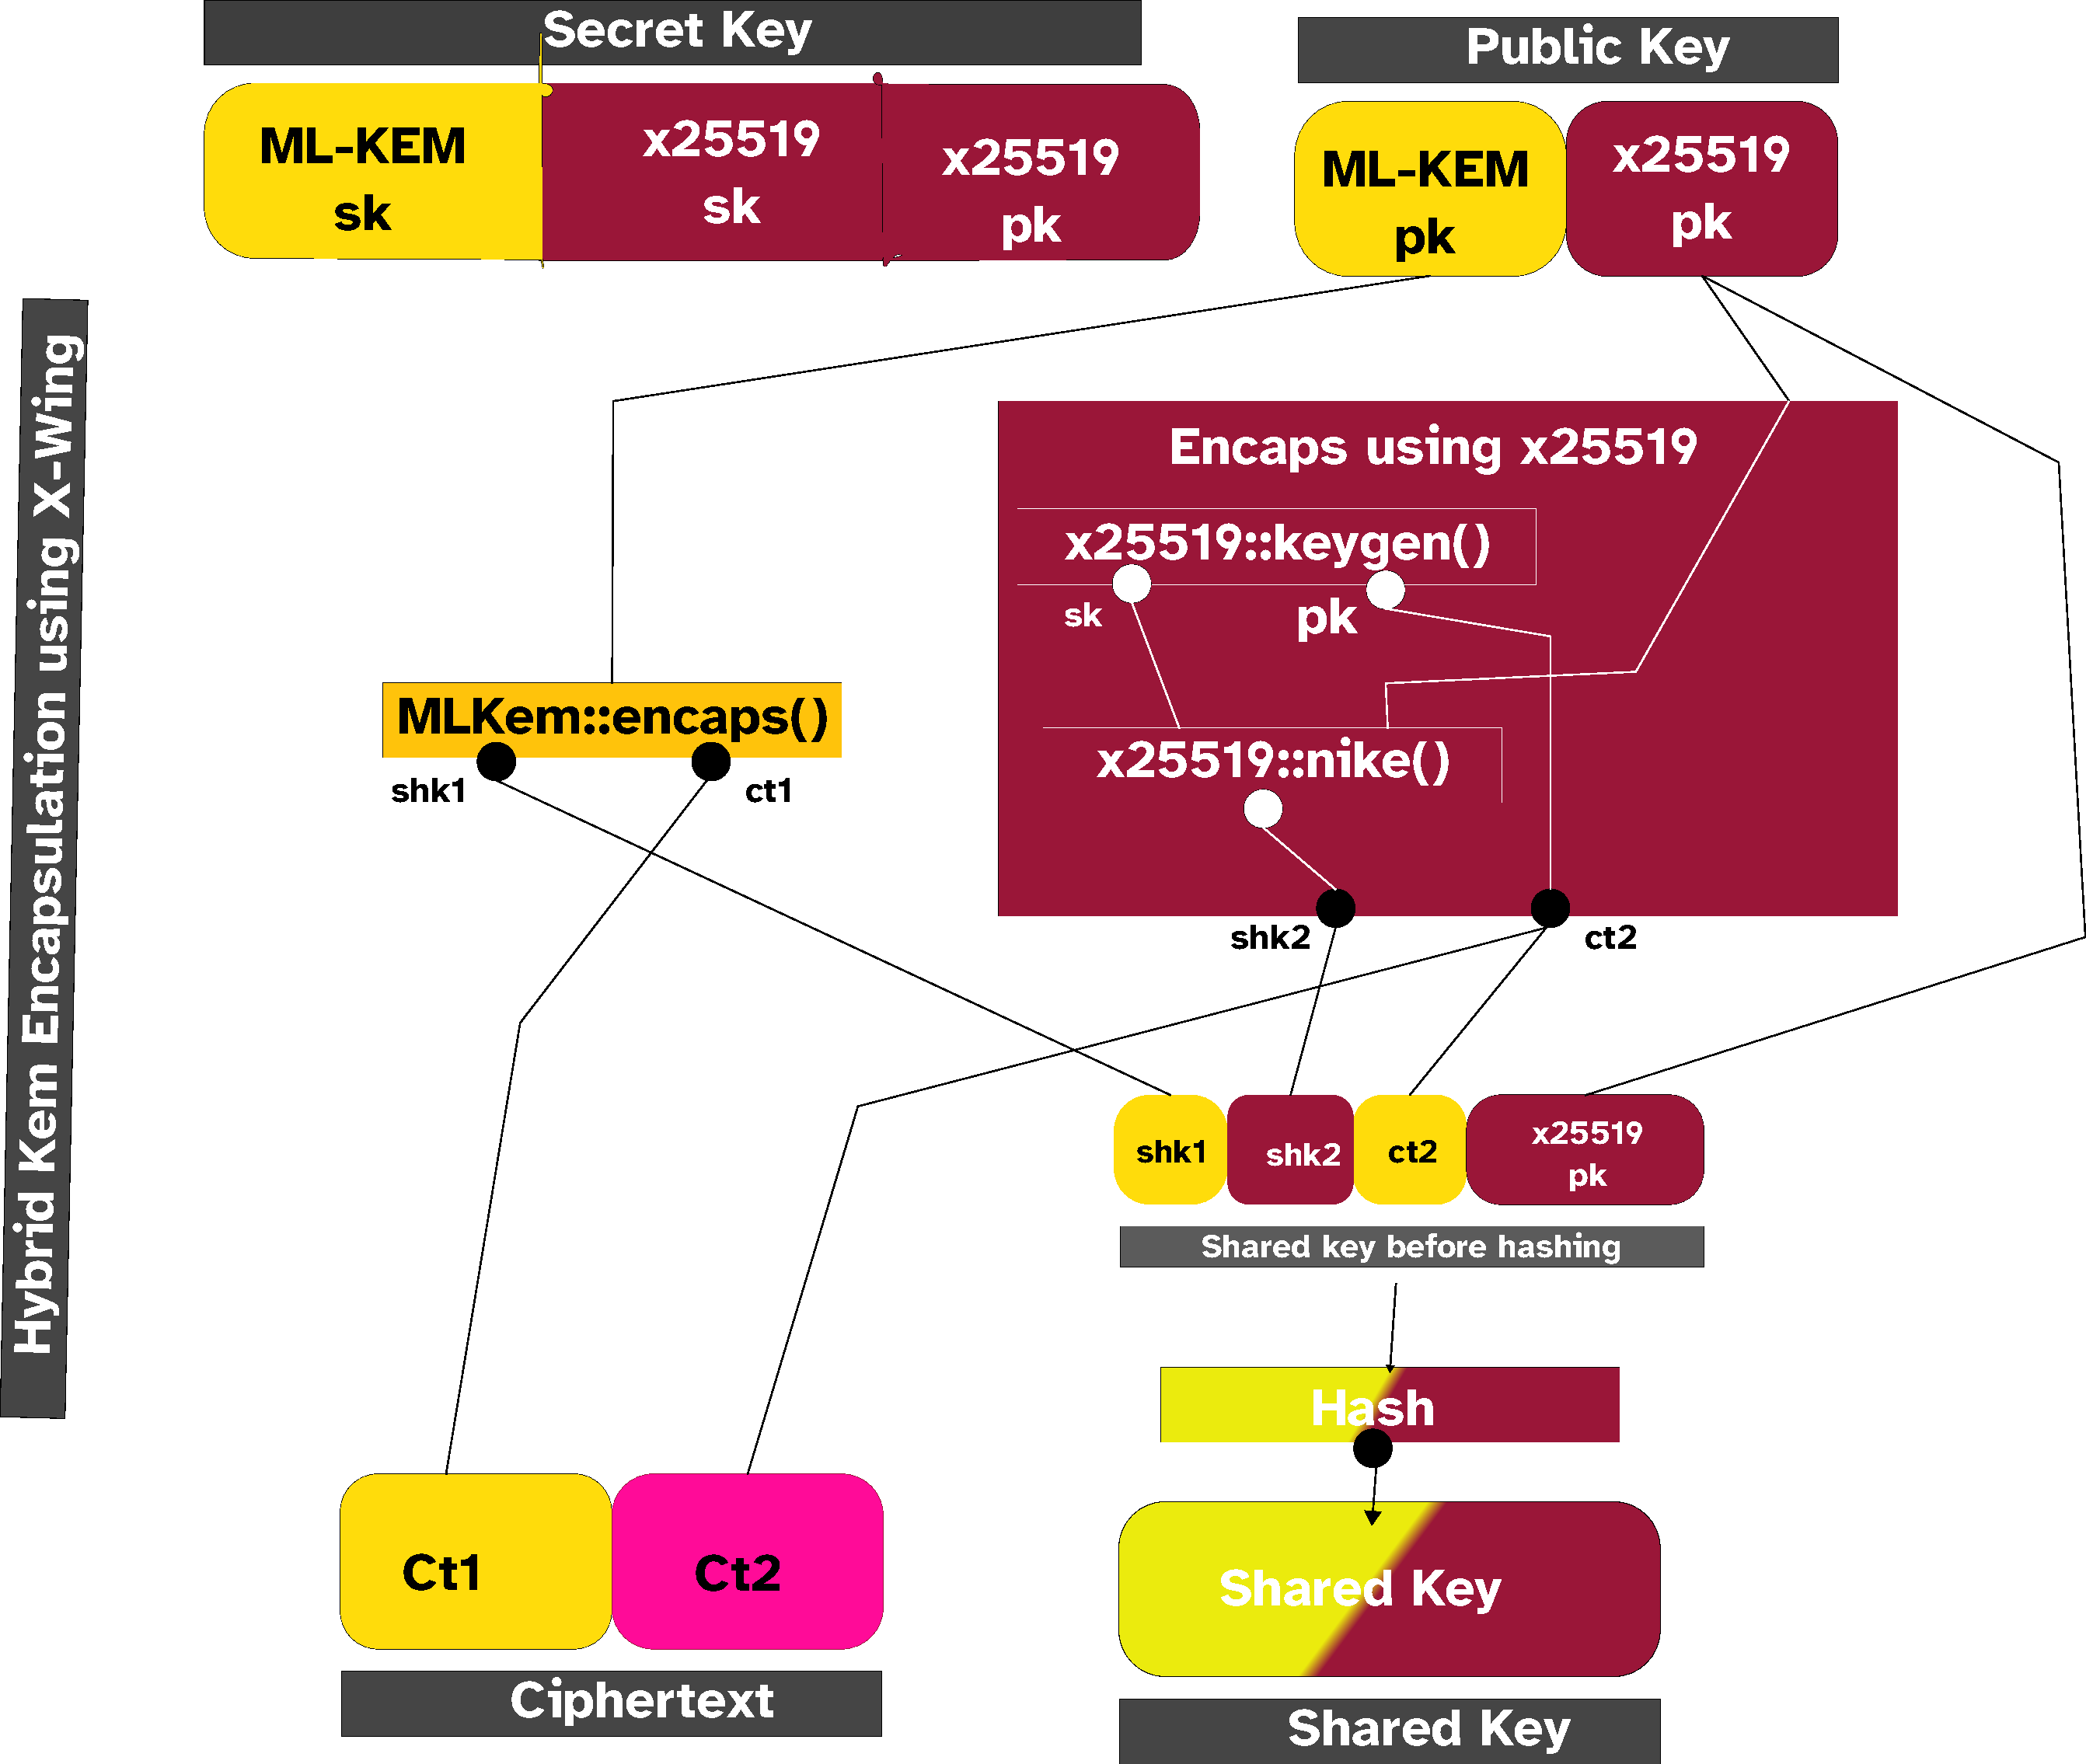
\includegraphics[height=.85\textheight]{graphics/xwing.pdf}
\end{frame}

\begin{frame}{Rosenpass \& WireGuard Hybridization}
  \hypertarget{hybrid-security-with-wireguard}{}
  \centering
  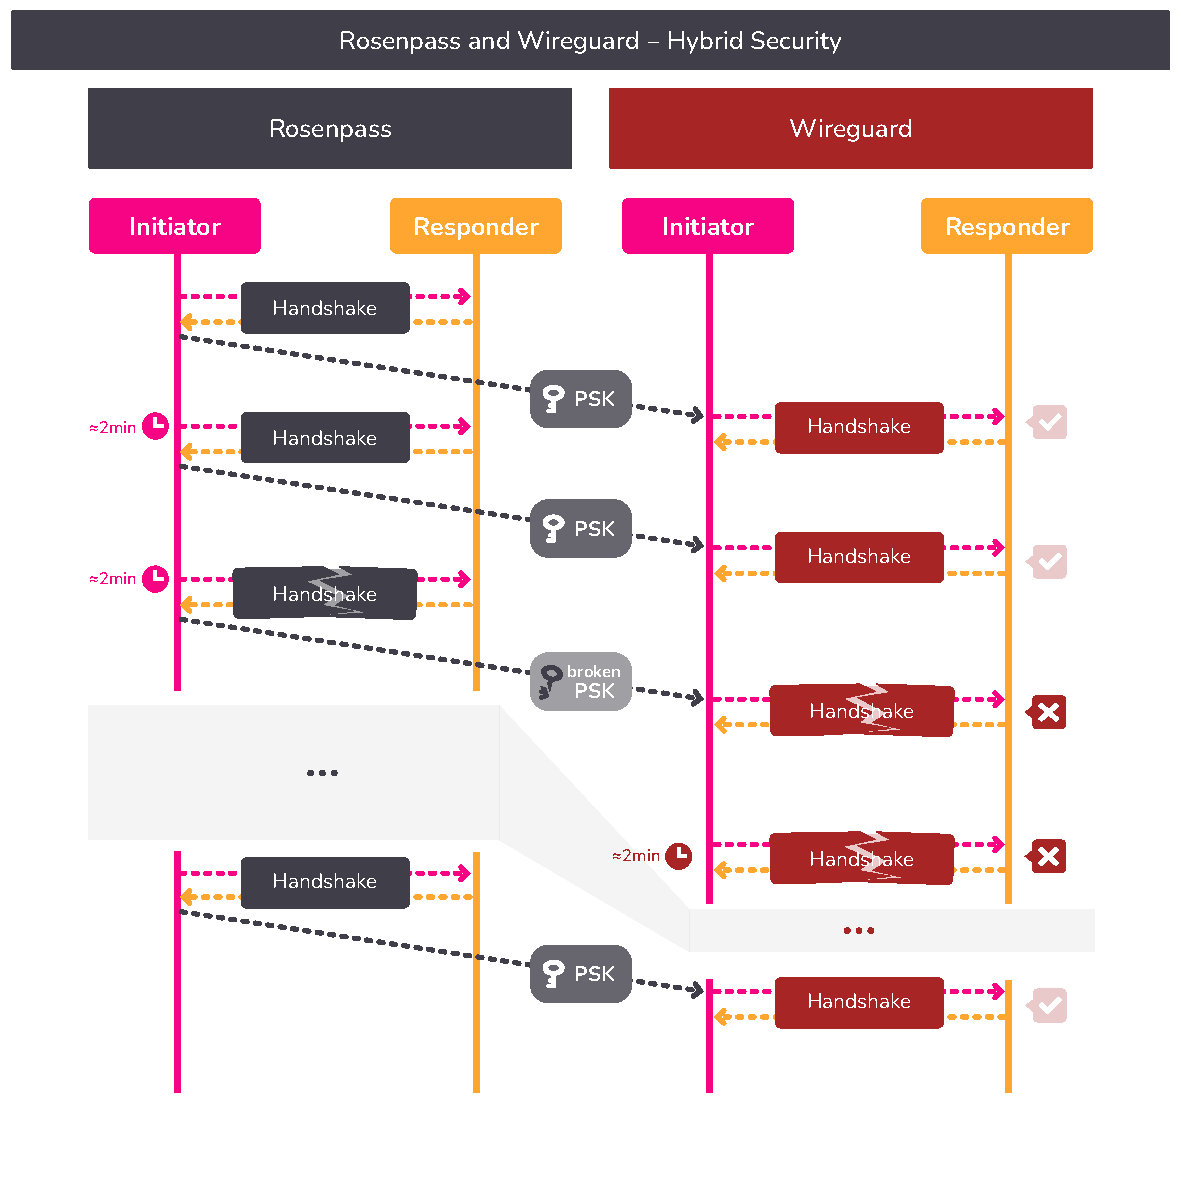
\includegraphics[height=1.03\textheight, clip=true,trim=0cm 0cm 0cm 3.2cm]{graphics/rosenpass-wireguard-hybrid-security.pdf}
\end{frame}
